\newpage
\section{Class \Iclass{circle}} % (fold)
\label{sec:class_circle}

\subsection{Attributes of a circle} % (fold)
\label{sub:attributes_of_a_circle}
This class is defined by two points: the center and a point through which the circle passes

\begin{mybox}
   Creation |C.OA = circle: new (z.O,z.A) |
\end{mybox}

\bgroup
\catcode`_=12
\small
\captionof{table}{Circle attributes.}\label{circle:att}
\begin{tabular}{lll}
\toprule
\textbf{Attributes}     & \textbf{Application} &\\
\Iattr{circle}{center}  & |z.A = C.AB.center| &\\
\Iattr{circle}{through} & |z.B = C.AB.through| &\\
\Iattr{circle}{type}    &  |C.AB.type|   &  |C.OA.type = 'circle'|\\
\Iattr{circle}{radius}  &  |C.AB.radius| &   |r = C.OA.radius | $r$ real number\\
\Iattr{circle}{north}   &  |C.AB.north|  &   |z.N = C.OA.north|\\
\Iattr{circle}{south}   &  |C.AB.south|  &    |z.S = C.OA.south| \\
\Iattr{circle}{east}    &  |C.AB.east|   &   |z.E = C.OA.east| \\
\Iattr{circle}{west}    &  |C.AB.west|   &   |z.W = C.OA.west| \\
\Iattr{circle}{opp}    &  |z.Ap = C.AB.opp|   & [\ref{ssub:example_circle_attributes}]  \\
\Iattr{circle}{ct}    &  |L = C.AB.ct|  [ \ref{ssub:example_circle_attributes} ]  \\
\bottomrule %
\end{tabular}
\egroup

\subsubsection{Example: circle attributes} % (fold)
\label{ssub:example_circle_attributes}

Three attributes are used (south, west, radius).  

\begin{minipage}{0.5\textwidth}
\begin{Verbatim}
\begin{tkzelements}
   scale = .5
   z.a   = point: new (1, 1)
   z.b   = point: new (5, 4)
   C.ab  = circle : new (z.a,z.b)
   z.s   = C.ab.south
   z.w   = C.ab.west
   r     = C.ab.radius
   z.c   = C.ab.opp
   z.r,z.t = get_points (C.ab.ct : ortho_from (z.b))
\end{tkzelements}
\begin{tikzpicture}
\tkzGetNodes
\tkzDrawPoints(a,b,c,s,w)
\tkzLabelPoints(a,b,c,s,w)
\tkzDrawCircle(a,b)
\tkzDrawSegments(a,b r,t b,c)
\tkzLabelSegment[sloped](a,b){ab = \tkzUseLua{r}}
\end{tikzpicture}
\end{Verbatim}
\end{minipage}
\begin{minipage}{0.5\textwidth}
\begin{tkzelements}
   scale = .5
   z.a = point: new (1, 1)
   z.b = point: new (5, 4)
   C.ab = circle : new (z.a,z.b)
   z.s = C.ab.south
   z.w = C.ab.west
   r   = C.ab.radius
   z.c   = C.ab.opp
   z.r,z.t = get_points (C.ab.ct : ortho_from (z.b))
\end{tkzelements}

\emph{\begin{tikzpicture}
\tkzGetNodes
\tkzDrawPoints(a,b,c,s,w)
\tkzLabelPoints(a,b,c,s,w)
\tkzDrawCircle(a,b)
\tkzDrawSegments(a,b r,t b,c)
\tkzLabelSegment[sloped](a,b){ab = \tkzUseLua{r}}
\end{tikzpicture}}

\end{minipage}
% subsubsection example_circle_attributes (end)
% subsection attributes_of_a_circle (end)

\newpage
\subsection{Methods of the class circle} % (fold)
\label{sub:methods_of_the_class_circle}
\bgroup
\catcode`_=12
\small
\captionof{table}{Circle methods.}\label{circle:met}
\begin{tabular}{lll}
\toprule
\textbf{Methods} & \textbf{Comments}   & \\
\midrule   \\
\Igfct{circle}{new(O,A)} & |C.OA = circle : new (z.O,z.A)| & center $O$ through $A$; [\ref{ssub:method_imeth_circle_new}]\\
\Igfct{circle}{radius(O,r)} & |C.OA = circle : radius (z.O,2)| & center $O$ radius =2 cm; [\ref{ssub:method_imeth_circle_radius}]\\
\Igfct{circle}{diameter(A,B)} & |C.OA = circle :diameter(z.A,z.B)| & diameter $[AB]$; [\ref{ssub:method_imeth_circle_diameter}]  \\
\midrule 
 \textbf{Points} &&\\
\midrule 
\Imeth{circle}{antipode (pt)} & |z.C = C.OA: antipode (z.B)| &    $[BC]$ = diameter;  [\ref{ssub:method_imeth_circle_antipode}]   \\
\Imeth{circle}{midarc (pt,pt)} & |z.D = C.AB: midarc (z.B,z.C)|& $D$ is the midarc of $\widearc{BC}$; [\ref{ssub:method_imeth_circle_midarc}]\\
\Imeth{circle}{point (r)} & |z.E = C.AB: point (0.25)|& |r| between 0 and 1;  [\ref{ssub:method_imeth_circle_point}]\\
\Imeth{circle}{random\_pt(lower, upper)} & &\\
\Imeth{circle}{inversion (obj)} & |z.Bp = C.AC: inversion (z.B)|& [\ref{ssub:inversion}]\\
\Imeth{circle}{internal\_similitude (C)} & |z.I= C.one: internal_similitude(C.two)| &  [\ref{ssub:method_imeth_circle_internal__similitude}]\\
\Imeth{circle}{external\_similitude (C)} & |z.J= C.one: external_similitude(C.two)| &  [\ref{ssub:method_imeth_circle_external__similitude}] \\ 
\Imeth{circle}{radical\_center (C1<,C2>)} & or only (C1) & [\ref{ssub:radical_center} ]  \\
\midrule 
 \textbf{Lines} & & \\
\midrule 
\Imeth{circle}{radical\_axis (C)} &   [ \ref{ssub:method_imeth_circle_radical__axis_c} ; \ref{sub:d_alembert_2} ] & \\
\Imeth{circle}{tangent\_at (pt)} & |z.P=C.OA:tangent_at(z.M)| & [\ref{ssub:method_imeth_circle_tangent}] \\
\Imeth{circle}{tangent\_from (pt)}& |z.M,z.N=C.OA: tangent_from (z.P)| & [\ref{ssub:method_imeth_circle_tangent} ] \\
\Imeth{circle}{common\_tangent (C)}& |z.a,z.b = C.AC: common_tangent (C.EF)|&  [\ref{ssub:common_tangent} ; \ref{sub:common_tangent_orthogonality}] \\
\midrule 
 \textbf{Circles}& &\\
\midrule 
\Imeth{circle}{orthogonal\_from (pt)}  &|C=C.OA:orthogonal_from (z.P)|  & [\ref{ssub:method_imeth_circle_orthogonal_from_pt} ;\ref{sub:altshiller} ; \ref{sub:pencil_v1}]  \\
\Imeth{circle}{orthogonal\_through(pta,ptb)}&|C=C.OA:orthogonal_through (z.z1,z.z2)| &  [\ref{ssub:method_imeth_circle_orthogonal_through}]\\
\Imeth{circle}{midcircle (C)}  & |C.inv = C.OA: midcircle (C.EF)|  & [\ref{ssub:midcircle}] \\
\Imeth{circle}{radical\_circle (C1<,C2>)} & or only (C1) &  [\ref{ssub:radical_circle}] \\
\midrule 
 \textbf{Miscellaneous} &&\\
\midrule 
\Imeth{circle}{power (pt)}     &| r = C.OA: power (z.M)| &  [\ref{par:power_v1} ; \ref{par:power_v2} ; \ref{sub:apollonius_circle_v1_with_inversion} ] \\
\Imeth{circle}{in\_out (pt)} & |C.OA : in_out (z.M)| & [\ref{ssub:in_out_for_circle_and_disk}]  \\
\Imeth{circle}{in\_out\_disk (pt)} & |C.OA : in_out_disk (z.M)| & [\ref{ssub:in_out_for_circle_and_disk}]  \\
\Imeth{circle}{draw ()} & for further use &\\
\Imeth{circle}{circles\_position (C1)} & result = string & [\ref{ssub:circles_position}] \\
\bottomrule 
\end{tabular}
\egroup
% subsection methods_circle (end)

\subsubsection{Method \Imeth{circle}{new}} % (fold)
\label{ssub:method_imeth_circle_new}

A circle is defined by its centre and a point through which it passes.

\vspace{6pt}
\begin{minipage}{.5\textwidth}
\begin{Verbatim}
\begin{tkzelements}
z.O     = point:    new (0,0)
z.A     = point:    new (2,1)
C       = circle:   new (z.O , z.A)
\end{tkzelements}
\begin{tikzpicture}[gridded]
\tkzGetNodes
\tkzDrawCircles(O,A)
\tkzDrawPoints(A,O)
\tkzLabelPoints[right](A,O)
\end{tikzpicture}
\end{Verbatim}
\end{minipage}
\begin{minipage}{.5\textwidth}
\begin{tkzelements}
z.O     = point:    new (0,0)
z.A     = point:    new (2,1)
C       = circle:   new (z.O , z.A)
\end{tkzelements}
  \begin{center}
\begin{tikzpicture}[gridded]
\tkzGetNodes
\tkzDrawCircles(O,A)
\tkzDrawPoints(A,O)
\tkzLabelPoints[right](A,O)
\end{tikzpicture}
  \end{center}

\end{minipage}

% subsubsection method_imeth_circle_new (end)

\subsubsection{Method \Imeth{circle}{radius}} % (fold)
\label{ssub:method_imeth_circle_radius}


We define a circle with its centre and radius.

\vspace{6pt}
\begin{minipage}{.5\textwidth}
\begin{Verbatim}
\begin{tkzelements}
z.O     = point:    new (0,0)
z.A     = point:    new (2,1)
C       = circle:   radius (z.A , math.sqrt(5))
z.T     = C.through 
\end{tkzelements}
\begin{tikzpicture}[gridded]
\tkzGetNodes
\tkzDrawCircles(A,T)
\tkzDrawPoints(A,O,T)
\tkzLabelPoints[right](A,O,T)
\end{tikzpicture}
\end{Verbatim}
\end{minipage}
\begin{minipage}{.5\textwidth}
  \begin{tkzelements}
  z.O     = point:    new (0,0)
  z.A     = point:    new (2,1)
  C       = circle:   radius (z.A , math.sqrt(5))
  z.T     = C.through 
  \end{tkzelements}
  \begin{center}
    \begin{tikzpicture}[gridded]
    \tkzGetNodes
    \tkzDrawCircles(A,T)
    \tkzDrawPoints(A,O,T)
    \tkzLabelPoints[right](A,O,T)
    \end{tikzpicture}
  \end{center}
\end{minipage}
% subsubsection method_imeth_circle_radius (end)

\subsubsection{Method \Imeth{circle}{diameter}} % (fold)
\label{ssub:method_imeth_circle_diameter}

A circle is defined by two points at the ends of one of its diameters.

\vspace{6pt}
\begin{minipage}{.5\textwidth}
\begin{Verbatim}
\begin{tkzelements}
z.A     = point:    new (0,0)
z.B     = point:    new (2,1)
C       = circle:   diameter (z.A , z.B)
z.O     = C.center
z.T     = C.through 
\end{tkzelements}
\begin{tikzpicture}[gridded]
\tkzGetNodes
\tkzDrawCircles(O,T)
\tkzDrawPoints(A,B,O,T)
\tkzLabelPoints[right](A,B,O,T)
\end{tikzpicture}
\end{Verbatim}
\end{minipage}
\begin{minipage}{.5\textwidth}
\begin{tkzelements}
z.A     = point:    new (0,0)
z.B     = point:    new (2,1)
C       = circle:   diameter (z.A , z.B)
z.O     = C.center
z.T     = C.through 
\end{tkzelements}
  \begin{center}
\begin{tikzpicture}[gridded]
\tkzGetNodes
\tkzDrawCircles(O,T)
\tkzDrawPoints(A,B,O,T)
\tkzLabelPoints[right](A,B,O,T)
\end{tikzpicture}
  \end{center}
\end{minipage}
% subsubsection method_imeth_circle_diameter (end)

\subsubsection{Method \Imeth{circle}{antipode}} % (fold)
\label{ssub:method_imeth_circle_antipode}
This method is used to define a point that is diametrically opposed to a point on a given circle.

\vspace{6pt}
\begin{minipage}{.5\textwidth}
\begin{Verbatim}
\begin{tkzelements}
z.A     = point:    new (0,0)
z.O     = point:    new (2,1)
C       = circle:   new (z.O , z.A)
z.B     = C : antipode (z.A)
\end{tkzelements}
\begin{tikzpicture}[gridded]
\tkzGetNodes
\tkzDrawCircles(O,A)
\tkzDrawPoints(A,B,O)
\tkzLabelPoints[right](A,B,O)
\end{tikzpicture}
\end{Verbatim}
\end{minipage}
\begin{minipage}{.5\textwidth}
\begin{tkzelements}
z.A     = point:    new (0,0)
z.O     = point:    new (2,1)
C       = circle:   new (z.O , z.A)
z.B     = C : antipode (z.A)
\end{tkzelements}
  \begin{center}
\begin{tikzpicture}[gridded]
\tkzGetNodes
\tkzDrawCircles(O,A)
\tkzDrawPoints(A,B,O)
\tkzLabelPoints[right](A,B,O)
\end{tikzpicture}
  \end{center}
\end{minipage}


% subsubsection method_imeth_circle_antipode (end)

\subsubsection{Method \Imeth{circle}{midarc}} % (fold)
\label{ssub:method_imeth_circle_midarc}
The definition given in [ \href{https://mathworld.wolfram.com/Mid-ArcPoints.html}{Weisstein, Eric W. "Mid-Arc Points." From MathWorld--A Wolfram Web Resource.}] is as follows:
The mid-arc points  of a triangle as defined by Johnson (1929) are the points on the circumcircle of the triangle which lie half-way along each of the three arcs determined by the vertices. These points arise in the definition of the Fuhrmann circle and Fuhrmann triangle, and lie on the extensions of the perpendicular bisectors of the triangle sides drawn from the circumcenter.

The definition I use here is more general: the defined point is simply the point that divides an arc into two arcs of the same length.

\vspace{6pt}
\begin{minipage}{.5\textwidth}
\begin{Verbatim}
\begin{tkzelements}
z.A     = point:    new (0,0)
z.O     = point:    new (2,1)
C       = circle:   new (z.O , z.A)
z.B     = C : point (0.25)
z.M     = C : midarc (z.A,z.B)
\end{tkzelements}
\begin{tikzpicture}[gridded]
\tkzGetNodes
\tkzDrawCircles(O,A)
\tkzDrawPoints(A,B,O,M)
\tkzLabelPoints[right](A,B,O,M)
\end{tikzpicture}
\end{Verbatim}
\end{minipage}
\begin{minipage}{.5\textwidth}
\begin{tkzelements}
z.A     = point:    new (0,0)
z.O     = point:    new (2,1)
C       = circle:   new (z.O , z.A)
z.B     = C : point (0.25)
z.M     = C : midarc (z.A,z.B)
\end{tkzelements}
  \begin{center}
\begin{tikzpicture}[gridded]
\tkzGetNodes
\tkzDrawCircles(O,A)
\tkzDrawPoints(A,B,O,M)
\tkzLabelPoints[right](A,B,O,M)
\end{tikzpicture}
  \end{center}
\end{minipage}

% subsubsection method_imeth_circle_midarc (end)

\subsubsection{Method \Imeth{circle}{point (r)}} % (fold)
\label{ssub:method_imeth_circle_point}

Let $C$ be a circle with centre $O$ and passing through $A$ such that |z.A = C.through|. This method defines a point $M$ on the circle from A such that the ratio of the length of $\widearc{AM}$ to the circumference of the circle is equal to $r$.

In the next example, $r=\dfrac{1}{6}$ corresponds to $\dfrac{\pi/3}{2\pi}$, so the angle $\widehat{AOE}$ has the measure $\pi/3$.

If $r=.5$ the defined point is diametrically opposed to $A$, the angle $\widehat{AOD}$ has the measure $\pi$.

\vspace{6pt}
\begin{minipage}{.5\textwidth}
\begin{Verbatim}
 \begin{tkzelements}
   z.O  = point:  new (0,0)
   z.A  = point:  new (1,2)
   C.OA = circle:  new (z.O,z.A)
   z.B = C.OA: point (1/6)
   z.C = C.OA: point (0.25)
   z.D = C.OA: point (0.5)
\end{tkzelements}
\begin{tikzpicture}
\tkzGetNodes
\tkzDrawCircle(O,A)
\tkzDrawPoints(A,...,D,O)
\tkzLabelPoints(A,...,D,O)
\end{tikzpicture}
\end{Verbatim}
\end{minipage}
\begin{minipage}{.5\textwidth}
 \begin{tkzelements}
   z.O  = point:  new (0,0)
   z.A  = point:  new (1,2)
   C.OA = circle:  new (z.O,z.A)
   z.B = C.OA: point (1/6)
   z.C = C.OA: point (0.25)
   z.D = C.OA: point (0.5)
\end{tkzelements}
\begin{center}
\begin{tikzpicture}
\tkzGetNodes
\tkzDrawCircle(O,A)
\tkzDrawPoints(A,...,D,O)
\tkzLabelPoints(A,...,D,O)
\end{tikzpicture}
\end{center}

\end{minipage}


% subsubsection method_imeth_circle_point (end)

\subsubsection{Method \Imeth{circle}{inversion (obj)}: point, line and circle} % (fold)
\label{ssub:inversion}

The \code{inversion} method can be used on a point, a line or a circle. Depending on the type of object, the function determines the correct algorithm to use.

\paragraph{Inversion: point} % (fold)
\label{par:inversion_point}

The \code{inversion} method can be used on a point, a group of points, a line or a circle. Depending on the type of object, the function determines the correct algorithm to use.

\begin{minipage}{.5\textwidth}
\begin{Verbatim}
\begin{tkzelements}
   z.o   = point:    new (-1,2)
   z.a   = point:    new (2,1)
   C.oa  = circle:   new (z.o,z.a)
   z.c   = point:    new (3,4)
   z.d   = C.oa:     inversion (z.c)
   p     = C.oa:     power (z.c)
\end{tkzelements}
\begin{tikzpicture}
    \tkzGetNodes   
    \tkzDrawCircle(o,a)
    \tkzDrawSegments(o,a o,c)
    \tkzDrawPoints(a,o,c,d)
    \tkzLabelPoints(a,o,c,d)
    \tkzLabelSegment[sloped,above=1em](c,d){%
    Power of c with respect to C is \tkzUseLua{p}}
 \end{tikzpicture}
\end{Verbatim}
\end{minipage}
\begin{minipage}{.5\textwidth}
\begin{tkzelements}
   scale =.75
   z.o   = point:    new (-1,2)
   z.a   = point:    new (2,1)
   C.oa  = circle:   new (z.o,z.a)
   z.c   = point:    new (3,4)
   z.d   = C.oa:     inversion (z.c)
   p     = C.oa:     power (z.c)
\end{tkzelements}

\begin{center}
  \begin{tikzpicture}
      \tkzGetNodes   
      \tkzDrawCircle(o,a)
      \tkzDrawSegments(o,a o,c)
      \tkzDrawPoints(a,o,c,d)
      \tkzLabelPoints(a,o,c,d)
      \tkzLabelSegment[sloped,above=1em](c,d){%
       La puissance de c est \tkzUseLua{p}}
   \end{tikzpicture}
\end{center}

\end{minipage}

\paragraph{Inversion: line} % (fold)
\label{par:inversion_line}

The result is either a straight line or a circle.

\begin{minipage}{.5\textwidth}
\begin{Verbatim}
\begin{tkzelements}
   z.o      = point:    new (-1,1)
   z.a      = point:    new (1,3)
   C.oa     = circle:   new (z.o,z.a)
   z.c      = point:    new (3,2)
   z.d      = point:    new (0,4)
   L.cd     = line:     new (z.c,z.d)
   C.OH     = C.oa: inversion (L.cd)
   z.O,z.H  = get_points(C.OH)
\end{tkzelements}
\begin{tikzpicture}
    \tkzGetNodes    
    \tkzDrawCircles(o,a O,H)
    \tkzDrawLines(c,d o,H)
    \tkzDrawPoints(a,o,c,d,H)
    \tkzLabelPoints(a,o,c,d,H)
 \end{tikzpicture}
\end{Verbatim}
\end{minipage}
\begin{minipage}{.5\textwidth}
\begin{tkzelements}
   z.o      = point:    new (-1,1)
   z.a      = point:    new (1,3)
   C.oa     = circle:   new (z.o,z.a)
   z.c      = point:    new (3,2)
   z.d      = point:    new (0,4)
   L.cd     = line:     new (z.c,z.d)
   C.OH     = C.oa: inversion (L.cd)
   z.O,z.H  = get_points(C.OH)
\end{tkzelements}

\begin{center}
  \begin{tikzpicture}
      \tkzGetNodes    
      \tkzDrawCircles(o,a)
      \tkzDrawCircles[new](O,H)
      \tkzDrawLines(c,d o,H)
      \tkzDrawPoints(a,o,c,d,H)
      \tkzLabelPoints(a,o,c,d,H)
   \end{tikzpicture}
\end{center}

\end{minipage}
 
\paragraph{Inversion: circle} % (fold)
 \label{par:inversion_circle}

The result is either a straight line or a circle.

\begin{minipage}{.55\textwidth}
\begin{Verbatim}
\begin{tkzelements}
scale = .7
z.o,z.a  = point:  new (-1,3),point:  new (2,3)
z.c      = point:  new (-2,1)
z.e,z.d  = point:  new (-2,7),point: new (-3,5)
C.oa     = circle: new (z.o,z.a)
C.ed     = circle: new (z.e,z.d)
C.co     = circle: new (z.c,z.o)
obj      = C.oa: inversion (C.co)
   if obj.type == "line"
   then z.p,z.q = get_points(obj)
   else z.f,z.b = get_points(obj) end
obj      = C.oa: inversion(C.ed)
if obj.type == "line"
then z.p,z.q = get_points(obj)
else z.f,z.b = get_points(obj) end
color = "orange"
\end{tkzelements}
\begin{tikzpicture}
\tkzGetNodes 
\tkzDrawCircles[black](o,a)
\tkzDrawCircles[teal](c,o e,d)
\tkzDrawCircles[\tkzUseLua{color}](f,b)
\tkzDrawLines[\tkzUseLua{color}](p,q)
\tkzDrawPoints(a,...,f,o,p,q)
\tkzLabelPoints(a,...,f,o,p,q)
\end{tikzpicture}
\end{Verbatim}
\end{minipage}
\begin{minipage}{.45\textwidth}
   \begin{tkzelements}
      scale = .7
      z.o,z.a  = point:  new (-1,3),point:  new (2,3)
      z.c      = point:  new (-2,1)
      z.e,z.d  = point:  new (-2,7),point: new (-3,5)
      C.oa     = circle: new (z.o,z.a)
      C.ed     = circle: new (z.e,z.d)
      C.co     = circle: new (z.c,z.o)
      obj      = C.oa: inversion (C.co)
         if obj.type == "line"
         then z.p,z.q = get_points(obj)
         else z.f,z.b = get_points(obj) end
      obj      = C.oa: inversion(C.ed)
         if obj.type == "line"
         then z.p,z.q = get_points(obj)
         else z.f,z.b = get_points(obj) end
      color = "orange"
   \end{tkzelements}

   \begin{center}
     \begin{tikzpicture}
         \tkzGetNodes 
         \tkzDrawCircles[black](o,a)
         \tkzDrawCircles[teal](c,o e,d)
         \tkzDrawCircles[\tkzUseLua{color}](f,b)
         \tkzDrawLines[\tkzUseLua{color}](p,q)
         \tkzDrawPoints(a,...,f,o,p,q)
        \tkzLabelPoints(a,...,f,o,p,q)
      \end{tikzpicture}
   \end{center}
\end{minipage}

% subsubsection inversion (end)

\subsubsection{Method \Imeth{circle}{internal\_similitude}} % (fold)
\label{ssub:method_imeth_circle_internal__similitude}

Circles are geometrically similar to one another and mirror symmetric. Hence, a pair of circles has both types of homothetic centers, internal and external, unless the centers are equal or the radii are equal; these exceptional cases are treated after general position. These two homothetic centers lie on the line joining the centers of the two given circles, which is called the line of centers. Circles with radius zero can also be included (see exceptional cases), and negative radius can also be used, switching external and internal. [Wikipedia]

\begin{minipage}{.5\textwidth}
\begin{Verbatim}
\begin{tkzelements}
  scale = 0.75
z.A  = point : new ( 0  , 0  )
z.a  = point : new ( 2 ,  2 )
z.B  = point : new ( 5  , 2  )
z.b  = point : new ( 6  , 1  )
C.Aa = circle : new (z.A,z.a)
C.Bb = circle : new (z.B,z.b)
z.I  = C.Aa : internal_similitude (C.Bb)
L.TA1,L.TA2 = C.Aa : tangent_from (z.I)
z.A1 = L.TA1.pb
z.A2 = L.TA2.pb
\end{tkzelements}
\begin{tikzpicture}
\tkzGetNodes
\tkzDrawCircles(A,a B,b)
\tkzDrawPoints(A,a,B,b,I,A1,A2)
\tkzDrawLines[add = 1 and 2](A1,I A2,I)
\end{tikzpicture}
\end{Verbatim}
\end{minipage}
\begin{minipage}{.5\textwidth}
\begin{tkzelements}
  scale = .75
z.A  = point : new ( 0  , 0  )
z.a  = point : new ( 2 ,  2 )
z.B  = point : new ( 5  , 2  )
z.b  = point : new ( 6  , 1  )
C.Aa = circle : new (z.A,z.a)
C.Bb = circle : new (z.B,z.b)
z.I  = C.Aa : internal_similitude (C.Bb)
L.TA1,L.TA2 = C.Aa : tangent_from (z.I)
z.A1 = L.TA1.pb
z.A2 = L.TA2.pb
\end{tkzelements}
\begin{center}
  \begin{tikzpicture}
  \tkzGetNodes
  \tkzDrawCircles(A,a B,b)
  \tkzDrawPoints(A,a,B,b,I,A1,A2)
  \tkzDrawLines[add = 1 and 2](A1,I A2,I)
  \end{tikzpicture}
\end{center}
\end{minipage}

% subsubsection method_imeth_circle_internal__similitude (end)

\subsubsection{Method \Imeth{circle}{external\_similitude}} % (fold)
\label{ssub:method_imeth_circle_external__similitude}

\begin{minipage}{.5\textwidth}
\begin{Verbatim}
\begin{tkzelements}
z.A  = point : new ( 0  , 0  )
z.a  = point : new ( 2 ,  2 )
z.B  = point : new ( 3  , 2  )
z.b  = point : new ( 4  , 1  )
C.Aa = circle : new (z.A,z.a)
C.Bb = circle : new (z.B,z.b)
z.I  = C.Aa : external_similitude (C.Bb)
L.TA1,L.TA2 = C.Aa : tangent_from (z.I)
z.A1 = L.TA1.pb
z.A2 = L.TA2.pb
\end{tkzelements}
\begin{tikzpicture}
\tkzGetNodes
\tkzDrawCircles(A,a B,b)
\tkzDrawPoints(A,a,B,b,I,A1,A2)
\tkzDrawLines[add = .5 and .2](A1,I A2,I)
\end{tikzpicture}
\end{Verbatim}
\end{minipage}
\begin{minipage}{.5\textwidth}
\begin{tkzelements}
  scale = .75
z.A  = point : new ( 0  , 0  )
z.a  = point : new ( 2 ,  2 )
z.B  = point : new ( 3  , 2  )
z.b  = point : new ( 4  , 1  )
C.Aa = circle : new (z.A,z.a)
C.Bb = circle : new (z.B,z.b)
z.I  = C.Aa : external_similitude (C.Bb)
L.TA1,L.TA2 = C.Aa : tangent_from (z.I)
z.A1 = L.TA1.pb
z.A2 = L.TA2.pb
\end{tkzelements}
\begin{center}
\begin{tikzpicture}
\tkzGetNodes
\tkzDrawCircles(A,a B,b)
\tkzDrawPoints(A,a,B,b,I,A1,A2)
\tkzDrawLines[add = .5 and .2](A1,I A2,I)
\end{tikzpicture}
\end{center}
\end{minipage}
% subsubsection method_imeth_circle_external__similitude (end)


\subsubsection{Method \Imeth{circle}{radical\_center (C1,C2)}} % (fold)
\label{ssub:radical_center}

The radical lines of three circles are concurrent in a point known as the radical center (also called the power center). This theorem was originally demonstrated by Monge (Dörrie 1965, p. 153). [\href{https://mathworld.wolfram.com/RadicalCenter.html}{Weisstein, Eric W. "Radical Center." From MathWorld--A Wolfram Web Resource. }
]

Here I have also named \code{radical\_center} the point of intersection of the radical axis of two circles with the centre axis. See the following example for how to obtain point $H$.


\begin{minipage}[t]{.5\textwidth}\vspace{0pt}%
\begin{Verbatim}
\begin{tkzelements}
   z.O      = point : new (0,0)
   z.x      = point : new (1,0)
   z.y      = point : new (4,0)
   z.z      = point : new (2,0)
   z.Op     = point : new (4,2)
   z.P      = point : new (2,2.5)
   C.Ox     = circle :    new (z.O,z.x)
   C.Pz     = circle :    new (z.P,z.z)
   C.Opy    = circle :    new (z.Op,z.y)
   z.ap,z.a = intersection (C.Ox,C.Pz)
   z.bp,z.b = intersection (C.Opy,C.Pz)
   L.aap    = line : new (z.a,z.ap)
   L.bbp    = line : new (z.b,z.bp)
   --  z.X      = intersection (L.aap,L.bbp)
   z.X      = C.Ox : radical_center(C.Pz,C.Opy)
   --   L.OOp    = line : new (z.O,z.Op)
   --   z.H      = L.OOp : projection (z.X)
   z.H = C.Ox : radical_center(C.Opy)
\end{tkzelements}
\begin{tikzpicture}
   \tkzGetNodes
   \tkzDrawCircles(O,a O',b P,z)
   \tkzDrawLines[red](a,X b',X H,X O,O')
   \tkzDrawPoints(O,O',P,a,a',b,b',X,H)
   \tkzLabelPoints[below right](O,O',P,H)
\end{tikzpicture}
\end{Verbatim}
\end{minipage}
\begin{minipage}[t]{.5\textwidth}\vspace{0pt}%
\begin{tkzelements}
z.O         = point : new (0,0)
z.x         = point : new (1,0)
z.y         = point : new (4,0)
z.z         = point : new (2,0)
z.Op        = point : new (4,2)
z.P         = point : new (2,2.5)
C.Ox        = circle :    new (z.O,z.x)
C.Pz        = circle :    new (z.P,z.z)
C.Opy       = circle :    new (z.Op,z.y)
z.ap,z.a    = intersection (C.Ox,C.Pz)
z.bp,z.b    = intersection (C.Opy,C.Pz)
L.aap       = line : new (z.a,z.ap)
L.bbp       = line : new (z.b,z.bp)
z.X         = intersection (L.aap,L.bbp)
L.OOp       = line : new (z.O,z.Op)
z.H         = L.OOp : projection (z.X)
\end{tkzelements}

\begin{center}
  \begin{tikzpicture}
  \tkzGetNodes
  \tkzDrawCircles(O,a O',b P,z)
  \tkzDrawLines[red](a,X b',X H,X O,O')
  \tkzDrawPoints(O,O',P,a,a',b,b',X,H)
  \tkzLabelPoints[below right](O,O',P,H)
  \end{tikzpicture}
\end{center}

\end{minipage}
% subsubsection radical_center (end)

\subsubsection{Method \Imeth{circle}{radical\_axis}(C)} % (fold)
\label{ssub:method_imeth_circle_radical__axis_c}

The radical line, also called the radical axis, is the locus of points of equal circle power with respect to two nonconcentric circles. By the chordal theorem, it is perpendicular to the line of centers (Dörrie 1965). [\href{https://mathworld.wolfram.com/RadicalLine.html}{Weisstein, Eric W. "Radical Line." From MathWorld--A Wolfram Web Resource.} ]

\vspace{6pt}
\paragraph{Radical axis v1} % (fold)
\label{par:radical_axis_v1}

\begin{Verbatim}
\begin{tkzelements}
scale    = .75
z.X      = point : new (0,0)
z.B      = point : new (2,2)
z.Y      = point : new (7,1)
z.Ap     = point : new (8,-1)
L.XY     = line :    new (z.X,z.Y)
C.XB     = circle : new (z.X,z.B)
C.YAp    = circle : new (z.Y,z.Ap)
z.E,z.F  = get_points (C.XB : radical_axis (C.YAp))
z.A      = C.XB : point (0.4)
T.ABAp   = triangle: new (z.A,z.B,z.Ap)
z.O      = T.ABAp.circumcenter
C.OAp    = circle : new (z.O,z.Ap)
_,z.Bp   = intersection (C.OAp,C.YAp)
L.AB     = line : new (z.A,z.B)
L.ApBp   = line : new (z.Ap,z.Bp)
z.M      = intersection (L.AB,L.ApBp)
z.H      = L.XY : projection (z.M)
\end{tkzelements}
\begin{tikzpicture}
   \tkzGetNodes
   \tkzDrawCircles(X,B Y,A')
   \tkzDrawArc[dashed,delta=30](O,A')(A)
   \tkzDrawPoints(A,B,A',B',M,H,X,Y,O,E,F)
   \tkzDrawLines[red](A,M A',M X,Y E,F)
   \tkzDrawLines[red,add=1 and 3](M,H)
\end{tikzpicture}
\end{Verbatim}

\begin{tkzelements}
scale    = .75
z.X      = point : new (0,0)
z.B      = point : new (2,2)
z.Y      = point : new (7,1)
z.Ap     = point : new (8,-1)
L.XY     = line :    new (z.X,z.Y)
C.XB     = circle : new (z.X,z.B)
C.YAp    = circle : new (z.Y,z.Ap)
z.E,z.F  = get_points (C.XB : radical_axis (C.YAp))
z.A      = C.XB : point (0.4)
T.ABAp   = triangle: new (z.A,z.B,z.Ap)
z.O      = T.ABAp.circumcenter
C.OAp    = circle : new (z.O,z.Ap)
_,z.Bp   = intersection (C.OAp,C.YAp)
L.AB     = line : new (z.A,z.B)
L.ApBp   = line : new (z.Ap,z.Bp)
z.M      = intersection (L.AB,L.ApBp)
z.H      = L.XY : projection (z.M)
\end{tkzelements}

\begin{center}
  \begin{tikzpicture}
  \tkzGetNodes
  \tkzDrawCircles(X,B Y,A')
  \tkzDrawArc[dashed,delta=30](O,A')(A)
  \tkzDrawPoints(A,B,A',B',M,H,X,Y,O,E,F)
  \tkzDrawLines[red](A,M A',M X,Y E,F)
  \tkzDrawLines[red,add=1 and 3](M,H)
  \end{tikzpicture}
\end{center}
% paragraph radical_axis_v1 (end)

\paragraph{Radical axis v2} % (fold)
\label{par:radical_axis_v2}

\begin{Verbatim}
\begin{tkzelements}
scale       = 1.25
z.O         = point : new (-1,0)
z.Op        = point : new (4,-1)
z.B         = point : new (0,2)
z.D         = point : new (4,0)
C.OB        = circle :    new (z.O,z.B)
C.OpD       = circle :    new (z.Op,z.D)
L.EF        = C.OB : radical_axis (C.OpD)
z.E,z.F     = get_points (L.EF)
z.M         = L.EF : point (.75)
L.MT,L.MTp  = C.OB : tangent_from (z.M)
_,z.T       = get_points (L.MT)
_,z.Tp      = get_points (L.MTp)
L.MK,L.MKp  = C.OpD : tangent_from (z.M)
_,z.K       = get_points (L.MK)
_,z.Kp      = get_points (L.MKp)
\end{tkzelements}
\begin{tikzpicture}
   \tkzGetNodes
   \tkzDrawCircles(O,B O',D)
   \tkzDrawLine(E,F)
   \tkzDrawLine[add=.5 and .5](O,O')
   \tkzDrawLines[add = 0 and .5](M,T M,T' M,K M,K')
   \tkzDrawCircle(M,T)
   \tkzDrawPoints(O,O',T,M,T',K,K')
   \tkzLabelPoints(O,O',T,T',K,K',M)
\end{tikzpicture}
\end{Verbatim}

\begin{tkzelements}
scale =1.25
z.O     = point : new (-1,0)
z.Op    = point : new (4,-1)
z.B     = point : new (0,2)
z.D     = point : new (4,0)
C.OB    = circle :    new (z.O,z.B)
C.OpD   = circle :    new (z.Op,z.D)
L.EF    = C.OB : radical_axis (C.OpD)
z.E,z.F = get_points (L.EF)
z.M     = L.EF : point (.75)
L.MT,L.MTp  = C.OB : tangent_from (z.M)
_,z.T = get_points (L.MT)
_,z.Tp = get_points (L.MTp)
L.MK,L.MKp  = C.OpD : tangent_from (z.M)
_,z.K = get_points (L.MK)
_,z.Kp = get_points (L.MKp)
\end{tkzelements}

\begin{center}
  \begin{tikzpicture}
  \tkzGetNodes
  \tkzDrawCircles(O,B O',D)
  \tkzDrawLine(E,F)
  \tkzDrawLine[add=.5 and .5](O,O')
  \tkzDrawLines[add = 0 and .5](M,T M,T' M,K M,K')
  \tkzDrawCircle(M,T)
  \tkzDrawPoints(O,O',T,M,T',K,K')
  \tkzLabelPoints(O,O',T,T',K,K',M)
  \end{tikzpicture}
\end{center}
% paragraph radical_axis_v2 (end)

\paragraph{Radical axis v3} % (fold)
\label{par:radical_axis_v3}

\begin{Verbatim}
   \begin{tkzelements}
   z.O      = point : new (0,0)
   z.B      = point : new (4,0)
   z.Op     = point : new (6,0)
   C.OB     = circle :    new (z.O,z.B)
   C.OpB    = circle :    new (z.Op,z.B)
   L.EF     = C.OB : radical_axis (C.OpB)
   z.E,z.F  = get_points(L.EF)
   z.M      = L.EF : point (0.2)
   L        = C.OB : tangent_from (z.M)
   _,z.T    = get_points (L)
   L        = C.OpB : tangent_from (z.M)
   _,z.Tp   = get_points (L)
\end{tkzelements}
\begin{tikzpicture}
   \tkzGetNodes
   \tkzDrawCircles(O,B O',B)
   \tkzDrawSegments(M,T M,T')
   \tkzDrawSegments(E,F)
   \tkzDrawLine[add=.5 and .5](O,O')
   \tkzDrawPoints(O,B,O',E,F,M,T,T')
   \tkzLabelPoints(O,O',B,E,F,T,T')
   \tkzDrawArc(M,T')(T)
\end{tikzpicture}
\end{Verbatim}

\begin{tkzelements}
z.O      = point : new (0,0)
z.B      = point : new (4,0)
z.Op     = point : new (6,0)
C.OB     = circle :    new (z.O,z.B)
C.OpB    = circle :    new (z.Op,z.B)
L.EF     = C.OB : radical_axis (C.OpB)
z.E,z.F  = get_points(L.EF)
z.M      = L.EF : point (0.2)
L        = C.OB : tangent_from (z.M)
_,z.T    = get_points (L)
L        = C.OpB : tangent_from (z.M)
_,z.Tp   = get_points (L)
\end{tkzelements}
 
\begin{center}
  \begin{tikzpicture}
  \tkzGetNodes
  \tkzDrawCircles(O,B O',B)
  \tkzDrawSegments(M,T M,T')
  \tkzDrawSegments(E,F)
  \tkzDrawLine[add=.5 and .5](O,O')
  \tkzDrawPoints(O,B,O',E,F,M,T,T')
  \tkzLabelPoints(O,O',B,E,F,T,T')
  \tkzDrawArc(M,T')(T)
  \end{tikzpicture}
\end{center}
% paragraph radical_axis_v3 (end)

\paragraph{Radical axis v4} % (fold)
\label{par:radical_axis_v4}

\begin{Verbatim}
\begin{tkzelements}
   z.O     = point : new (0,0)
   z.B     = point : new (5,0)
   z.Op    = point : new (3,0)
   C.OB    = circle :    new (z.O,z.B)
   C.OpB   = circle :    new (z.Op,z.B)
   L.EF    = C.OB : radical_axis (C.OpB)
   z.E,z.F = get_points(L.EF)
   z.H     = L.EF.mid
   z.M     = L.EF : point (.8)
   _,L     = C.OB : tangent_from (z.M)
   _,z.T   = get_points (L)
   _,L     = C.OpB : tangent_from (z.M)
   _,z.Tp  = get_points (L)
\end{tkzelements}
\begin{tikzpicture}
   \tkzGetNodes
   \tkzDrawCircles(O,B O',B)
   \tkzDrawSegments(M,T M,T')
   \tkzDrawSegments(E,F)
   \tkzDrawLine[add=.3 and .3](O,H)
   \tkzDrawPoints(O,O',B,E,H,M)
   \tkzLabelPoints[below right](O,O',E,F,M,T,T')
   \tkzDrawArc(M,B)(T)
\end{tikzpicture}
\end{Verbatim}

\begin{tkzelements}
   z.O     = point : new (0,0)
   z.B     = point : new (5,0)
   z.Op    = point : new (3,0)
   C.OB    = circle :    new (z.O,z.B)
   C.OpB   = circle :    new (z.Op,z.B)
   L.EF    = C.OB : radical_axis (C.OpB)
   z.E,z.F = get_points(L.EF)
   z.H     = L.EF.mid
   z.M     = L.EF : point (.8)
   _,L     = C.OB : tangent_from (z.M)
   _,z.T   = get_points (L)
   _,L     = C.OpB : tangent_from (z.M)
   _,z.Tp  = get_points (L)
\end{tkzelements}

\begin{center}
  \begin{tikzpicture}
     \tkzGetNodes
     \tkzDrawCircles(O,B O',B)
     \tkzDrawSegments(M,T M,T')
     \tkzDrawSegments(E,F)
     \tkzDrawLine[add=.3 and .3](O,H)
     \tkzDrawPoints(O,O',B,E,H,M)
     \tkzLabelPoints[below right](O,O',E,F,M,T,T')
     \tkzDrawArc(M,B)(T)
  \end{tikzpicture}
\end{center}
% paragraph radical_axis_v4 (end)

% subsubsection method_imeth_circle_radical__axis_c (end)


\subsubsection{Methods \Imeth{circle}{tangent\_at (P)} and  \Imeth{circle}{tangent\_from (P)}} % (fold)
\label{ssub:method_imeth_circle_tangent}

\begin{minipage}{.5\textwidth}
\begin{Verbatim}
 \begin{tkzelements}
   z.A  = point:  new (0,0)
   z.B  = point:  new (1,2)   
   C.AB = circle: new (z.A,z.B)
   z.C  = point:  new (3,-2)
   L.T  = C.AB : tangent_at (z.B)
   z.D  = L.T.pb
   L.T1,L.T2 = C.AB : tangent_from (z.C)
   z.T1 = L.T1.pb
   z.T2 = L.T2.pb
\end{tkzelements}
\begin{tikzpicture}
\tkzGetNodes
\tkzDrawCircle(A,B)
\tkzDrawLines[add =.5 and .5](B,D C,T1 C,T2)
\tkzDrawSegments[dashed](A,B A,T1 A,T2)
\tkzDrawPoints(A,...,D,T1,T2)
\tkzLabelPoints[below left](A,T2,C)
\tkzLabelPoints[above right](B,T1,D)
\tkzMarkRightAngles(A,B,D A,T1,C A,T2,C)
\end{tikzpicture}
\end{Verbatim}
\end{minipage}
\begin{minipage}{.5\textwidth}
 \begin{tkzelements}
   z.A  = point:  new (0,0)
   z.B  = point:  new (1,2)   
   C.AB = circle: new (z.A,z.B)
   z.C  = point:  new (3,-2)
   L.T  = C.AB : tangent_at (z.B)
   z.D  = L.T.pb
   L.T1,L.T2 = C.AB : tangent_from (z.C)
   z.T1 = L.T1.pb
   z.T2 = L.T2.pb
\end{tkzelements}
\begin{center}
  \begin{tikzpicture}
  \tkzGetNodes
  \tkzDrawCircle(A,B)
  \tkzDrawLines[add =.5 and .5](B,D C,T1 C,T2)
  \tkzDrawSegments[dashed](A,B A,T1 A,T2)
  \tkzDrawPoints(A,...,D,T1,T2)
  \tkzLabelPoints[below left](A,T2,C)
  \tkzLabelPoints[above right](B,T1,D)
  \tkzMarkRightAngles(A,B,D A,T1,C A,T2,C)
  \end{tikzpicture}
\end{center}

\end{minipage}
% subsubsection  (end)

\subsubsection{Common tangent: Angle of two intersecting circles} % (fold)
\label{ssub:common_tangent}

Let be a tangent common to both circles at $T$ and $T'$ (closest to $C$). Let a secant parallel to this tangent pass through $C$. Then the segment $[TT']$ is seen from the other common point $D$ at an angle equal to half the angle of the two circles.

\begin{Verbatim}
\begin{tkzelements}
   z.A   = point : new ( 0  , 0  )
   z.B   = point : new ( 5  , 2  )
   L.AB = line : new ( z.A , z.B )
   z.C   = point : new ( 1 , 2 )
   C.AC  = circle : new (z.A,z.C)
   C.BC  = circle : new (z.B,z.C)
   z.T,z.Tp = C.AC : common_tangent (C.BC)
   L.TTp = line : new (z.T,z.Tp)
   z.M   = C.AC : point (0.45)
   L.MC  =line : new (z.M,z.C)
   z.Mp  = intersection (L.MC, C.BC) 
   L.mm = L.TTp : ll_from (z.C)
   _,z.M = intersection (L.mm, C.AC)
   z.Mp = intersection (L.mm, C.BC)
   _,z.D = intersection (C.AC,C.BC)
\end{tkzelements}         
\begin{tikzpicture}
   \tkzGetNodes
   \tkzDrawCircles(A,C B,C)
   \tkzDrawSegments(M,M' A,D B,D A,B C,D T,C T',C)
   \tkzDrawSegments[gray](D,M D,M' T,T' D,T D,T')
   \tkzDrawPoints(A,B,C,D,M,M',T,T')
   \tkzLabelPoints(A,B,D,M)
   \tkzLabelPoints[above](C,M',T,T')
   \tkzMarkAngles[mark=|,size=.75](T,C,M C,T,T' C,D,T T,D,M)
   \tkzMarkAngles[mark=||,size=.75](M',C,T' T,T',C T',D,C M',D,T')
\end{tikzpicture}
\end{Verbatim}


\begin{tkzelements}
z.A   = point : new ( 0  , 0  )
z.B   = point : new ( 5  , 2  )
L.AB = line : new ( z.A , z.B )
z.C   = point : new ( 1 , 2 )
C.AC  = circle : new (z.A,z.C)
C.BC  = circle : new (z.B,z.C)
z.T,z.Tp = C.AC : common_tangent (C.BC)
L.TTp = line : new (z.T,z.Tp)
z.M   = C.AC : point (0.45)
L.MC  =line : new (z.M,z.C)
z.Mp  = intersection (L.MC, C.BC) 
L.mm = L.TTp : ll_from (z.C)
_,z.M = intersection (L.mm, C.AC)
z.Mp = intersection (L.mm, C.BC)
_,z.D = intersection (C.AC,C.BC)
\end{tkzelements}
    
\begin{center}
  \begin{tikzpicture}
  \tkzGetNodes
  \tkzDrawCircles(A,C B,C)
  \tkzDrawSegments(M,M' A,D B,D A,B C,D T,C T',C)
  \tkzDrawSegments[gray](D,M D,M' T,T' D,T D,T')
  \tkzDrawPoints(A,B,C,D,M,M',T,T')
  \tkzLabelPoints(A,B,D,M)
  \tkzLabelPoints[above](C,M',T,T')
  \tkzMarkAngles[mark=|,size=.75](T,C,M C,T,T' C,D,T T,D,M)
  \tkzMarkAngles[mark=||,size=.75](M',C,T' T,T',C T',D,C M',D,T')
  \end{tikzpicture}
\end{center}
% subsubsection common_tangent (end)

\subsubsection{Method \Imeth{circle}{orthogonal\_from (pt)}} % (fold)
\label{ssub:method_imeth_circle_orthogonal_from_pt}

In geometry, two circles are said to be orthogonal if their respective tangent lines at the points of intersection are perpendicular (meet at a right angle). [wikipedia]

This method determines a circle with a given centre, orthogonal to a circle that is also given.

\begin{Verbatim}
\begin{tkzelements}
   scale    = .6
   z.C_1    = point: new (0,0)
   z.C_2    = point: new (8,0)
   z.A      = point: new (5,0)
   C        = circle: new (z.C_1,z.A)
   z.S,z.T  = get_points (C: orthogonal_from (z.C_2))
\end{tkzelements}
\begin{tikzpicture}
   \tkzGetNodes
   \tkzDrawCircles(C_1,T C_2,T)
   \tkzDrawSegments(C_1,T C_2,T)
   \tkzDrawLine(C_1,C_2)
   \tkzMarkRightAngle[fill=teal,%
  opacity=.2,size=1](C_1,T,C_2)
   \tkzDrawPoints(C_1,C_2,T)
   \tkzLabelPoints(C_1,C_2)
   \tkzLabelPoints[above](T)
   \tkzLabelSegment[left](C_1,T){r}
   \tkzLabelSegments[right](C_2,T){$\gamma$}
   \tkzLabelSegment[below](C_1,C_2){d}
   \tkzLabelCircle[left=10pt](C_1,T)(180){Circle 1}
   \tkzLabelCircle[right=10pt](C_2,T)(180){Circle 2}
\end{tikzpicture}
\end{Verbatim}

\begin{tkzelements}
scale    = .6
z.C_1    = point: new (0,0)
z.C_2    = point: new (8,0)
z.A  = point: new (5,0)
C    = circle: new (z.C_1,z.A)
z.S,z.T  = get_points (C: orthogonal_from (z.C_2))
\end{tkzelements}

\begin{center}
  \begin{tikzpicture}
  \tkzGetNodes
  \tkzDrawCircles(C_1,T C_2,T)
  \tkzDrawSegments(C_1,T C_2,T)
  \tkzDrawLine(C_1,C_2)
  \tkzMarkRightAngle[fill=teal,opacity=.2,size=.5](C_1,T,C_2)
  \tkzDrawPoints(C_1,C_2,T)
  \tkzLabelPoints(C_1,C_2)
  \tkzLabelPoints[above](T)
  \tkzLabelSegment[left](C_1,T){r}
  \tkzLabelSegments[right](C_2,T){$\gamma$}
  \tkzLabelSegment[below](C_1,C_2){d}
  \tkzLabelCircle[left=10pt](C_1,T)(180){Circle 1}
  \tkzLabelCircle[right=10pt](C_2,T)(180){Circle 2}
  \end{tikzpicture}
\end{center}

% subsubsection method_imeth_circle_orthogonal__from_pt (end)

\subsubsection{Method \Imeth{circle}{orthogonal\_through}} % (fold)
\label{ssub:method_imeth_circle_orthogonal_through}

\begin{minipage}{.5\textwidth}
\begin{Verbatim}
\begin{tkzelements}
   z.O   = point: new (0,1)
   z.A   = point: new (1,0)
   z.z1  = point: new (-1.5,-1.5)
   z.z2  = point: new (2.5,-1.25)
   C.OA  = circle: new (z.O,z.A)
   C     = C.OA: orthogonal_through (z.z1,z.z2)
   z.c   = C.center
\end{tkzelements}
\begin{tikzpicture}
   \tkzGetNodes
   \tkzDrawCircle(O,A)
   \tkzDrawCircle[new](c,z1)
   \tkzDrawPoints[new](O,A,z1,z2,c)
   \tkzLabelPoints[right](O,A,z1,z2,c)
\end{tikzpicture}
\end{Verbatim}
\end{minipage}
\begin{minipage}{.5\textwidth}\begin{tkzelements}
   z.O   = point: new (0,1)
   z.A   = point: new (1,0)
   z.z1  = point: new (-1.5,-1.5)
   z.z2  = point: new (2.5,-1.25)
   C.OA  = circle: new (z.O,z.A)
   C = C.OA: orthogonal_through (z.z1,z.z2)
   z.c   = C.center
\end{tkzelements}

\begin{center}
  \begin{tikzpicture}
  \tkzGetNodes
  \tkzDrawCircle(O,A)
  \tkzDrawCircle[orange](c,z1)
  \tkzDrawPoints[orange](O,A,z1,z2,c)
  \tkzLabelPoints[right](O,A,z1,z2,c)
  \end{tikzpicture}
\end{center}
\end{minipage}
% subsubsection method_imeth_circle_orthogonal__through (end)

\subsubsection{midcircle} % (fold)
\label{ssub:midcircle}

\begin{minipage}{0.95\linewidth }
\emph{From Eric Danneels and Floor van Lamoen: A midcircle of two given circles is a circle that swaps the two given circles by inversion. Midcircles are in the same pencil of circles as the given circles.  The center of the midcircle(s) is one or both of the centers of similitude. We can distinguish four cases:
\begin{enumerate}[label=(\roman*)]
   \item  The two given circles intersect: there are two midcircles with centers at the centers of similitude of the given circles;
   \item One given circle is in the interior of the other given circle. Then there is one midcircle with center of similitude at the internal center of similitude of the given circles;
   \item One given circle is in the exterior of the other given circle. Then there is one midcircle with center at the external center of similitude of the given circles.
Clearly the tangency cases can be seen as limit cases of the above;
\item  If the circles intersect in a single point, the unique midcircle has center at the external similitude center or at internal similitude center. 
\end{enumerate} }
\end{minipage}

\vspace{1em}
Let's look at each of these cases:
\begin{enumerate}[label=(\roman*)]
\item If the two given circles intersect, then there are two  circles of inversion through their common points, with centers at the centers of similitudes.  The two midcircles bisect their angles and are orthogonal to each other. The centers of the midcircles are the internal center of similitude and the external center of similitude $I$ and $J$.

Consider two intersecting circles $(\mathcal{A})$ and $(\mathcal{B})$.
We can obtain the centers of similarity of these two circles by constructing $EH$ and $FG$ two diameters parallel of the circles $(\mathcal{A})$ and $(\mathcal{B})$. The  line $(GE)$ intercepts  the line $(AB)$ in $J$ and the line $(EF)$ intercepts the line $(AB)$ in $I$. The circles $(\mathcal{I})$ and $(\mathcal{J})$ are orthogonal and are the midcircles of $(\mathcal{A})$ and $(\mathcal{B})$. The division $(A,B;I,J)$ is harmonic.

\begin{minipage}{.4\textwidth}
\begin{Verbatim}
\begin{tkzelements}
scale = .8
z.A = point : new ( 1 , 0 ) 
z.B = point : new ( 3 , 0 ) 
z.O = point : new ( 2.1, 0 ) 
z.P = point : new ( 1 ,0 ) 
C.AO = circle : new (z.A,z.O)
C.BP = circle : new (z.B,z.P)
z.E = C.AO.south
z.H = C.AO.north
z.F = C.BP.north
z.G = C.BP.south
C.IT,C.JV = C.AO : midcircle (C.BP)
z.I,z.T = get_points (C.IT) 
z.J,z.V = get_points (C.JV) 
z.X,z.Y = intersection (C.AO,C.BP)
\end{tkzelements}  
\end{Verbatim}
\end{minipage}
\begin{minipage}{.6\textwidth}
   \begin{tkzelements}
   scale = .8
   z.A = point : new ( 1 , 0 ) 
   z.B = point : new ( 3 , 0 ) 
   z.O = point : new ( 2.1, 0 ) 
   z.P = point : new ( 1 ,0 ) 
   C.AO = circle : new (z.A,z.O)
   C.BP = circle : new (z.B,z.P)
   z.E = C.AO.south
   z.H = C.AO.north
   z.F = C.BP.north
   z.G = C.BP.south
   C.IT,C.JV = C.AO : midcircle (C.BP)
   z.I,z.T = get_points (C.IT) 
   z.J,z.V = get_points (C.JV) 
   z.X,z.Y = intersection (C.AO,C.BP)
   \end{tkzelements}
   \begin{tikzpicture}
   \tkzGetNodes
      \tkzDrawCircles[teal,thick](A,O B,P)
      \tkzDrawSegments[dashed,red](E,F I,B I,G I,F)
      \tkzDrawLines[gray](I,T J,V)
      \tkzDrawCircles[teal,thick](A,O B,P)
       \tkzDrawCircles[red,thick](I,X J,X)
      \tkzDrawPoints(A,B,I,J,E,F,G,H,X,Y)
      \tkzDrawPoints[red](I,J)
      \begin{scope}[font = \scriptsize]
      \tkzLabelPoints(A,I,J,G)
      \tkzLabelPoints[below left](E)
       \tkzLabelPoints[right](B)
       \tkzLabelPoints[above](F,H,X)
         \tkzLabelPoints[above right](Y)
      \end{scope}
   \end{tikzpicture}
\end{minipage}


\vfill

\item  One given circle is in the interior of the other given circle.
\label{midcircle_diameter}
\begin{minipage}{.6\textwidth}
\begin{Verbatim}
   \begin{tkzelements}
      scale =.75  
   z.A = point : new ( 3 , 0 ) 
   z.B = point : new ( 5 , 0 ) 
   z.O = point : new ( 2 , 0 ) 
   z.P = point : new ( 1 , 0 ) 
   L.AB = line :  new (z.A,z.B)
   C.AO = circle : new (z.A,z.O)
   C.BP = circle : new (z.B,z.P)
   z.R,z.S = intersection (L.AB,C.BP)
   z.U,z.V = intersection (L.AB,C.AO) 
   C.SV = circle  :  diameter (z.S,z.V)
   C.UR = circle  :  diameter (z.U,z.R)
   z.x = C.SV.center
   z.y = C.UR.center
   C.IT = C.AO : midcircle (C.BP)
   z.I,z.T = get_points (C.IT) 
\end{tkzelements}
\end{Verbatim}
\end{minipage}
\begin{minipage}{.6\textwidth}
   \begin{tkzelements}
         scale =.75  
      z.A = point : new ( 3 , 0 ) 
      z.B = point : new ( 5 , 0 ) 
      z.O = point : new ( 2 , 0 ) 
      z.P = point : new ( 1 , 0 ) 
      L.AB = line :  new (z.A,z.B)
      C.AO = circle : new (z.A,z.O)
      C.BP = circle : new (z.B,z.P)
      z.R,z.S = intersection (L.AB,C.BP)
      z.U,z.V = intersection (L.AB,C.AO) 
      C.SV = circle  :  diameter (z.S,z.V)
      C.UR = circle  :  diameter (z.U,z.R)
      z.x = C.SV.center
      z.y = C.UR.center
      C.IT = C.AO : midcircle (C.BP)
      z.I,z.T = get_points (C.IT) 
   \end{tkzelements}
   \begin{tikzpicture}
   \tkzGetNodes
      \tkzDrawCircles[teal,thick](A,O B,P)
      \tkzDrawCircles[green!20!black](x,S y,R)
      \tkzDrawPoints(A,B)
      \tkzDrawPoints[red](I)
      \tkzLabelPoints(A,B,I)
      \tkzDrawCircles[red,thick](I,T)
      \tkzLabelCircle[below](x,V)(270){$(\alpha)$}
      \tkzLabelCircle[below](y,R)(270){$(\beta)$} 
      \tkzLabelCircle[below](I,T)(250){$\textcolor{red}{(\gamma)}$}  
   \end{tikzpicture}  
   \end{minipage}

This case is a little more complicated. We'll construct the two circles $(\alpha)$ and $(\beta)$ tangent to the two given circles. Then we construct the radical circle orthogonal to the circles $(\alpha)$ and $(\beta)$. Its center is the radical center as well as the center of internal similtude of circles of center $A$ and $B$.

\item When the two given circles are external to each other,  we  construct  the external center of similitude of the two given circles.
$I$ is the center of external similarity of the two given circles. To obtain the inversion circle, simply note that $H$ is such that $IH^2= IE\times IF$. \label{tangent_from}

\begin{minipage}{.4\textwidth}
\begin{Verbatim}
\begin{tkzelements}
scale=.75
local a,b,c,d
z.A = point : new ( 0 , 0 )
z.B = point : new ( 4 , 0 )
z.a = point :  new ( .5 , 0)
z.b = point :  new ( 1 , 0)
C.Aa = circle  :  new (z.A,z.a)
C.Bb = circle  :  new (z.B,z.b)
L.AB = line :  new (z.A,z.B)
z.E = C.Aa.north
z.F = C.Bb.north
L.EF = line :  new (z.E,z.F)
C.IT =  C.Aa : midcircle (C.Bb)
z.I,z.T = get_points (C.IT) 
L.TF = C.Bb : tangent_from (z.I)
z.H = intersection (L.TF,C.IT)
z.E = intersection (L.TF,C.Aa)
z.F=L.TF.pb
\end{tkzelements}
\end{Verbatim}
\end{minipage}
\begin{minipage}{.6\textwidth}
\begin{tkzelements}
scale=.75
local a,b,c,d
z.A = point : new ( 0 , 0 )
z.B = point : new ( 4 , 0 )
z.a = point :  new ( .5 , 0)
z.b = point :  new ( 1 , 0)
C.Aa = circle  :  new (z.A,z.a)
C.Bb = circle  :  new (z.B,z.b)
L.AB = line :  new (z.A,z.B)
z.E = C.Aa.north
z.F = C.Bb.north
L.EF = line :  new (z.E,z.F)
C.IT =  C.Aa : midcircle (C.Bb)
z.I,z.T = get_points (C.IT) 
L.TF = C.Bb : tangent_from (z.I)
z.H = intersection (L.TF,C.IT)
z.E = intersection (L.TF,C.Aa)
z.F=L.TF.pb
\end{tkzelements}
\begin{tikzpicture}
\tkzGetNodes
\tkzDrawCircles[teal,thick](A,a B,b)
\tkzDrawCircles[red,thick](I,T) 
\tkzDrawSegments[gray](I,F)
\tkzDrawPoints(A,B,E,F)
\tkzDrawPoints[red](I,H) 
\tkzDrawLine(I,B)  
\tkzLabelPoints(A,B) 
\tkzLabelPoints[above](E,F) 
\tkzLabelPoints[above left,red](I,H) 
\end{tikzpicture}  
\end{minipage}


\item Consider two tangent circles $(\mathcal{A})$ and $(\mathcal{B})$,
\begin{itemize}

\item $(\mathcal{B})$ being external and angent to $(\mathcal{A})$. The construction is identical to the previous one.

\begin{minipage}{.4\textwidth}
\begin{Verbatim}
\begin{tkzelements}
scale=.75
local a,b,c,d
z.A = point : new ( 0 , 0 )
z.B = point : new ( 4 , 0 )
z.a = point :  new ( 1 , 0)
z.b = point :  new ( 1 , 0)
C.Aa = circle  :  new (z.A,z.a)
C.Bb = circle  :  new (z.B,z.b)
L.AB = line :  new (z.A,z.B)
z.E = C.Aa.north
z.F = C.Bb.north
L.EF = line :  new (z.E,z.F)
C.IT =  C.Aa : midcircle (C.Bb)
z.I,z.T = get_points(C.IT) 
L.TF = C.Bb : tangent_from (z.I)
z.H = intersection (L.TF,C.IT)
z.E = intersection (L.TF,C.Aa)
z.F=L.TF.pb
\end{tkzelements}
\end{Verbatim}
\end{minipage}
\begin{minipage}{.6\textwidth}
\begin{tkzelements}
scale=.75
local a,b,c,d
z.A = point : new ( 0 , 0 )
z.B = point : new ( 4 , 0 )
z.a = point :  new ( 1 , 0)
z.b = point :  new ( 1 , 0)
C.Aa = circle  :  new (z.A,z.a)
C.Bb = circle  :  new (z.B,z.b)
L.AB = line :  new (z.A,z.B)
z.E = C.Aa.north
z.F = C.Bb.north
L.EF = line :  new (z.E,z.F)
C.IT =  C.Aa : midcircle (C.Bb)
z.I,z.T = get_points (C.IT) 
L.TF = C.Bb : tangent_from (z.I)
z.H = intersection (L.TF,C.IT)
z.E = intersection (L.TF,C.Aa)
z.F=L.TF.pb
\end{tkzelements}
\begin{tikzpicture}
\tkzGetNodes
\tkzDrawCircles[teal,thick](A,a B,b)
\tkzDrawCircles[red,thick](I,T) 
\tkzDrawSegments[gray](I,F)
\tkzDrawPoints(A,B,E,F)
\tkzDrawPoints[red](I,H) 
\tkzDrawLine(I,B)  
\tkzLabelPoints(A,B) 
\tkzLabelPoints[above](E,F) 
\tkzLabelPoints[above left,red](I,H) 
\end{tikzpicture}  
\end{minipage}


\item   When one of the given circles is inside and tangent to the other, the construction is easy. 

\begin{minipage}{.4\textwidth}
\begin{Verbatim}
\begin{tkzelements}
z.A     = point : new ( 2 , 0 )
z.B     = point : new ( 4 , 0 )
z.a     = point :  new ( 1 , 0)
z.b     = point :  new ( 1 , 0)
C.Aa    = circle  :  new (z.A,z.a)
C.Bb    = circle  :  new (z.B,z.b)
C.IT    =  C.Aa : midcircle (C.Bb)
z.I,z.T  = get_points(C.IT)
\end{tkzelements}
\end{Verbatim}
\end{minipage}
\begin{minipage}{.6\textwidth}
\begin{tkzelements}
z.A = point : new ( 2 , 0 )
z.B = point : new ( 4 , 0 )
z.a = point :  new ( 1 , 0)
z.b = point :  new ( 1 , 0)
C.Aa = circle  :  new (z.A,z.a)
C.Bb = circle  :  new (z.B,z.b)
C.IT =  C.Aa : midcircle (C.Bb)
z.I,z.T = get_points (C.IT) 
\end{tkzelements}

\begin{tikzpicture}
\tkzGetNodes
\tkzDrawCircles[teal,thick](A,a B,b)
\tkzDrawCircles[red,thick](I,T) 
\tkzDrawPoints(A,B)  
\tkzDrawPoints[red](I) 
\tkzLabelPoints(A,B)  
\tkzLabelPoints[above left,red](I) 
\end{tikzpicture} 
\end{minipage}
\end{itemize}
\end{enumerate}

% subsubsection midcircle (end)


\subsubsection{Radical circle} % (fold)
\label{ssub:radical_circle}

\begin{minipage}[t]{.5\textwidth}\vspace{0pt}%
\begin{Verbatim} 
\begin{tkzelements}
   scale       = .5
   z.A         = point: new (0,0)
   z.B         = point: new (6,0)
   z.C         = point: new (0.8,4)
   T.ABC       = triangle : new ( z.A,z.B,z.C ) 
   C.exa       = T.ABC : ex_circle ()
   z.I_a,z.Xa  = get_points (C.exa)
   C.exb       = T.ABC : ex_circle (1)
   z.I_b,z.Xb  = get_points (C.exb)
   C.exc       = T.ABC : ex_circle (2)
   z.I_c,z.Xc  = get_points (C.exc)
   C.ortho     = C.exa : radical_circle (C.exb,C.exc)
   z.w,z.a     = get_points (C.ortho)
\end{tkzelements}
\begin{tikzpicture}
   \tkzGetNodes
   \tkzDrawPolygon(A,B,C)
   \tkzDrawCircles(I_a,Xa I_b,Xb I_c,Xc)
   \tkzDrawCircles[red,thick](w,a)
   \tkzDrawPoints(A,B,C)
   \tkzLabelPoints(A,B,C)
\end{tikzpicture}
\end{Verbatim}
\end{minipage}

\begin{tkzelements}
   scale       = .5
   z.A         = point: new (0,0)
   z.B         = point: new (6,0)
   z.C         = point: new (0.8,4)
   T.ABC       = triangle : new ( z.A,z.B,z.C ) 
   C.exa       = T.ABC : ex_circle ()
   z.I_a,z.Xa  = get_points (C.exa)
   C.exb       = T.ABC : ex_circle (1)
   z.I_b,z.Xb  = get_points (C.exb)
   C.exc       = T.ABC : ex_circle (2)
   z.I_c,z.Xc  = get_points (C.exc)
   C.ortho     = C.exa : radical_circle (C.exb,C.exc)
   z.w,z.a     = get_points (C.ortho)
\end{tkzelements}

\begin{center}
  \begin{tikzpicture}
     \tkzGetNodes
     \tkzDrawPolygon(A,B,C)
     \tkzDrawCircles(I_a,Xa I_b,Xb I_c,Xc)
     \tkzDrawCircles[red,thick](w,a)
     \tkzDrawPoints(A,B,C)
     \tkzLabelPoints(A,B,C)
  \end{tikzpicture}
\end{center}
% subsubsection radical_circle (end)

\subsubsection{Method \Imeth{circle}{power(C)}} % (fold)
\label{ssub:method_imeth_circle_power_c}

\paragraph{Power v1} % (fold)
\label{par:power_v1}
\begin{minipage}[t]{.5\textwidth}\vspace{0pt}%
\begin{Verbatim}
\begin{tkzelements}
   z.O     = point : new (0,0)
   z.A     = point : new (2,-2)
   z.M     = point : new (-6,0)
   L.AM    = line : new (z.A,z.M)
   C.OA    = circle :    new (z.O,z.A)
   z.Ap    = C.OA : antipode (z.A)
   z.B     = intersection (L.AM, C.OA)
\end{tkzelements}
\begin{tikzpicture}
   \tkzGetNodes
   \tkzDrawCircle(O,A)
   \tkzMarkRightAngle[fill=gray!10](A',B,M)
   \tkzDrawSegments(M,O A,A' A',B)
   \tkzDrawPoints(O,A,A',M,B)
   \tkzLabelPoints(O,A,A',M,B)
   \tkzDrawSegments[-Triangle](M,A M,A')
\end{tikzpicture}
\end{Verbatim}
\end{minipage}
\begin{minipage}[t]{.5\textwidth}
\begin{tkzelements}
scale = 1
z.O   = point : new (0,0)
z.A   = point : new (2,-2)
z.M   = point : new (-6,0)
L.AM  = line : new (z.A,z.M)
C.OA  = circle : new (z.O,z.A)
z.Ap  = C.OA : antipode (z.A)
z.B   = intersection (L.AM, C.OA)
\end{tkzelements}


\begin{center}
  \begin{tikzpicture}
  \tkzGetNodes
  \tkzDrawCircle(O,A)
  \tkzMarkRightAngle[fill=gray!10](A',B,M)
  \tkzDrawSegments(M,O A,A' A',B)
  \tkzDrawPoints(O,A,A',M,B)
  \tkzLabelPoints(O,A,A',M,B)
  \tkzDrawSegments[-Triangle](M,A M,A')
  \end{tikzpicture}
\end{center}

\end{minipage}
% paragraph power_v1 (end)

\paragraph{Power v2} % (fold)
\label{par:power_v2}
\begin{minipage}[t]{.5\textwidth}\vspace{0pt}%
\begin{Verbatim}
\begin{tkzelements}
   z.O     = point : new (0,0)
   z.A     = point : new (2,2)
   z.M     = point : new (-1.5,0)
   L.AM    = line : new (z.A,z.M)
   C.OA    = circle :    new (z.O,z.A)
   z.Ap    = C.OA : antipode (z.A)
   _,z.B   = intersection (L.AM, C.OA)
   z.m     = z.M : north(1)
   L.mM    = line : new (z.m,z.M)
   z.U,z.V = intersection (L.mM,C.OA)
\end{tkzelements}
\begin{tikzpicture}
   \tkzGetNodes
   \tkzDrawCircle(O,A)
   \tkzMarkRightAngle[fill=gray!10](A',B,M)
   \tkzDrawSegments(M,O A,A' A',B A,B U,V)
   \tkzDrawPoints(O,A,A',M,B,U,V,m)
   \tkzLabelPoints(O,A,M,U,V,m)
   \tkzLabelPoints[below left](A',B)
   \tkzDrawSegments(M,A M,A')
\end{tikzpicture}
\end{Verbatim}
\end{minipage}
\begin{minipage}[t]{.5\textwidth}\vspace{0pt}%
\begin{tkzelements}
scale = 1
z.O     = point : new (0,0)
z.A     = point : new (2,2)
z.M     = point : new (-1.5,0)
L.AM    = line : new (z.A,z.M)
C.OA    = circle :    new (z.O,z.A)
z.Ap    = C.OA : antipode (z.A)
_,z.B   = intersection (L.AM, C.OA)
z.m     = z.M : north(1)
L.mM    = line : new (z.m,z.M)
z.U,z.V = intersection (L.mM,C.OA)
\end{tkzelements}

\begin{center}
  \begin{tikzpicture}
  \tkzGetNodes
  \tkzDrawCircle(O,A)
  \tkzMarkRightAngle[fill=gray!10](A',B,M)
  \tkzDrawSegments(M,O A,A' A',B A,B U,V)
  \tkzDrawPoints(O,A,A',M,B,U,V,m)
  \tkzLabelPoints(O,A,M,U,V,m)
  \tkzLabelPoints[below left](A',B)
  \tkzDrawSegments(M,A M,A')
  \end{tikzpicture}
\end{center}

\end{minipage}
% paragraph power_v2 (end)

% subsubsection method_imeth_circle_power_c (end)

\subsubsection{Method \Imeth{circle}{in\_out} for circle and disk} % (fold)
\label{ssub:in_out_for_circle_and_disk}

\begin{minipage}{.5\textwidth}
  \begin{Verbatim}
  \begin{tkzelements}
  z.O = point : new (0,0)
  z.A = point : new (1,2)
  C.OA = circle : new (z.O,z.A)
  z.N = point : new (-2,2)
  z.M = point : new (1,0)
  z.P = point : new (2,1)
  BCm = C.OA : in_out (z.M)
  BDm = C.OA : in_out_disk (z.M)
  BCn = C.OA : in_out (z.N)
  BDn = C.OA : in_out_disk (z.N)
  BCp = C.OA : in_out (z.P)
  BDp = C.OA : in_out_disk (z.P)
  \end{tkzelements}
\end{Verbatim}
\end{minipage}
\begin{minipage}{.5\textwidth}\begin{tkzelements}
z.O = point : new (0,0)
z.A = point : new (1,2)
C.OA = circle : new (z.O,z.A)
z.N = point : new (-2,2)
z.M = point : new (1,0)
z.P = point : new (2,1)
BCm = C.OA : in_out (z.M)
BDm = C.OA : in_out_disk (z.M)
BCn = C.OA : in_out (z.N)
BDn = C.OA : in_out_disk (z.N)
BCp = C.OA : in_out (z.P)
BDp = C.OA : in_out_disk (z.P)
\end{tkzelements}
\def\tkzPosPoint#1#2#3#4{%
\tkzLabelPoints(O,M,N,P)
   \ifthenelse{\equal{\tkzUseLua{#1}}{true}}{
   \tkzLabelPoint[below=#4pt,font=\scriptsize](#2){on  the #3}}{%
   \tkzLabelPoint[below=#4pt,font=\scriptsize](#2){out  the #3}}
}    
\begin{center}
  \begin{tikzpicture}
  \tkzGetNodes
  \tkzDrawSegments[dashed](O,M O,N O,P)
  \tkzDrawCircle(O,A)
  \tkzDrawPoints(O,M,N,P)
  \tkzPosPoint{BCm}{M}{circle}{8}
  \tkzPosPoint{BCn}{N}{circle}{8}
  \tkzPosPoint{BCp}{P}{circle}{8}
  \tkzPosPoint{BDm}{M}{disk}{14}
  \tkzPosPoint{BDn}{N}{disk}{14}
  \tkzPosPoint{BDp}{P}{disk}{14}
  \end{tikzpicture}
\end{center}
\end{minipage}

\begin{minipage}{.5\textwidth}
  \begin{Verbatim}
  \def\tkzPosPoint#1#2#3#4{%
  \tkzLabelPoints(O,M,N,P)
     \ifthenelse{\equal{\tkzUseLua{#1}}{true}}{
     \tkzLabelPoint[below=#4pt,font=\scriptsize](#2){on  the #3}}{%
     \tkzLabelPoint[below=#4pt,font=\scriptsize](#2){out  the #3}}}    
  \begin{tikzpicture}
  \tkzGetNodes
  \tkzDrawSegments[dashed](O,M O,N O,P)
  \tkzDrawCircle(O,A)
  \tkzDrawPoints(O,M,N,P)
  \tkzPosPoint{BCm}{M}{circle}{8}
  \tkzPosPoint{BCn}{N}{circle}{8}
  \tkzPosPoint{BCp}{P}{circle}{8}
  \tkzPosPoint{BDm}{M}{disk}{14}
  \tkzPosPoint{BDn}{N}{disk}{14}
  \tkzPosPoint{BDp}{P}{disk}{14}
  \end{tikzpicture}
  \end{Verbatim}
\end{minipage}

% subsubsection in_out_for_circle_and_disk (end)

\subsubsection{Method \Imeth{circle}{circles\_position}} % (fold)
\label{ssub:circles_position}

This function returns a string indicating the position of the circle in relation to another. Useful for creating a function. Cases are:

\begin{itemize}
   \item \code{outside}
   \item \code{outside tangent}
   \item \code{inside tangent}
   \item \code{inside}
   \item \code{intersect}
\end{itemize}

\begin{minipage}{.5\textwidth}
\begin{Verbatim}
\begin{tkzelements}
   z.A      = point : new ( 0  , 0  )
   z.a      = point : new ( 3  , 0  )
   z.B      = point : new ( 2  , 0  )
   z.b      = point : new ( 3  , 0  )
   C.Aa     = circle: new (z.A,z.a)
   C.Bb     = circle: new (z.B,z.b)
   position = C.Aa : circles_position (C.Bb)
   if position == "inside tangent" 
   then color = "orange" 
   else color = "blue" end
\end{tkzelements}
       
\begin{tikzpicture}
   \tkzGetNodes
   \tkzDrawCircle(A,a)
   \tkzDrawCircle[color=\tkzUseLua{color}](B,b)
\end{tikzpicture}
\end{Verbatim}
\end{minipage}
\begin{minipage}{.5\textwidth}
\begin{tkzelements}
z.A = point : new ( 1  , 0  )
z.a = point : new ( 3  , 0  )
z.B = point : new ( 2  , 0  )
z.b = point : new ( 3  , 0  )
C.Aa = circle: new (z.A,z.a)
C.Bb = circle: new (z.B,z.b)
position = C.Aa : circles_position (C.Bb)
if position == "inside tangent" then color = "orange" else color = "blue" end
\end{tkzelements}
\hspace{\fill}
\begin{tikzpicture}
\tkzGetNodes
\tkzDrawCircle(A,a)
\tkzDrawCircle[color=\tkzUseLua{color}](B,b)
\end{tikzpicture}\hspace{\fill}
\end{minipage}
% subsubsection circles__position (end)

% subsection methods_of_the_class_circle (end)
% section class_circle (end)

\endinput
